\documentclass[11pt]{article}

%4pp das transps
% psnup -W415 -H273 -s.9 -b10 -d10 -c -4 05-Tecnicas_Compressao_Imagens.ps 05-Tecnicas_Compressao_Imagens.4pp.ps

\usepackage[utf8]{inputenc} % PARA USAR PALAVRAS EM PORT
\usepackage[portuguese]{babel}
\usepackage{a4wide}
\usepackage{color}
\usepackage{colordvi}
\usepackage{epsf,epsfig}
\usepackage{amsmath}
\usepackage{amsfonts}
\usepackage{enumerate}

\begin{document} 

\title{Lista de Exercícios de Sistemas de TV -- 2019-1}
\author{Luiz Feliep da S. Coelho \\ lfscoelho@ieee.org \\ DETEL -- UERJ \\ Departamento de Engenharia Eletrônica e Telecomunicações \\ Universidade do Estado do Rio de Janeiro}

\maketitle


\section{Aliasing em Imagens Digitais}

\textbf{Objetivo:} O principal objetivo das atividades desta seção é verificar empiricamente aspectos relativos à amostragem espacial de imagens e o fenômeno do \emph{Aliasing} -- sobreposição espectral. Temos ainda o emprego de filtros bidimensionais. O secundário é expandir os conhecimentos sobre manipulação de matrizes e exibição de imagens usando o \textsf{Matlab}.

\subsection{Geração de \emph{Zoneplates}}

\begin{enumerate}

\item \textbf{Tarefa:} Gere uma imagem $I$ cujos pixeis de coordenadas $(l,c)$ têm valores:

\begin{equation}
I(l, c) = \frac{1}{2} \cos{\left [  \frac{\beta \pi}{2M}\left (l^2 + c^2 \right ) \right ]} \label{eq:zoneplate}
\end{equation}
onde $-M/2 + 0.5 \leq l, c \leq M/2 - 0.5$.

\noindent Uma imagem assim gerada se chama um ``zoneplate'' e é bastante usada na avaliação de sistemas de processamento de imagens.

\begin{enumerate}

\item Fazer $\beta = 1$, $M = 256$ e apresentar a imagem (não esqueça de empregar o comando \textsf{truesize}).

\item Repetir o item anterior para $\beta = 0.5$ e $\beta = 2$. 

\item Compare as três imagens obtidas.

\end{enumerate}

\begin{itemize}
\item[\textit{Dica}:] Use o comando \textsf{meshgrid} para facilitar a geração dessas imagens.
\end{itemize}

\item \textbf{Pergunta:} O que você observa? 

Três imagens de ciculos concentricos, cuja frequência de alternância preto/branco aumenta de acordo com a distância do centro. Nesses locais com alta frequência são formadas ilusões de circulos.

\item \textbf{Pergunta:} O que pode ser dito a respeito do conteúdo de frequência dessas imagens?

De acordo com a distância do centro da imagem, a frequência aumenta. O termo $\beta$ está diretamente relacionado com a frequência das imagens. Com o aumentos de $\beta$ a frequência das imagens aumentam mais rapidamente.

\item \textbf{Pergunta:} Observe as imagens geradas a diferentes distâncias do monitor, como 2, 3, 4, 6 e 8H (sendo H é a altura do monitor). Qual a sua conclusão? Explique.

Com o aumento da distância, a ilusão fica mais evidente. Isso porque o sistema visual humano é incapaz de observar altas frequências e observa apenas os efeitos causados por ela.

\begin{itemize}
\item[\textit{Dica}:] Substitua $r^2 = l^2 + c^2$ na equação (\ref{eq:zoneplate}) e a partir disso calcule a frequência espacial em função de $r$. Vimos anteriormente como fazer isto.
\end{itemize}

\item \textbf{Pergunta:} Qual a influência de $\beta$ na frequência espacial da imagem?

O aumento de $\beta$ aumenta o quão rápido a frequência aumenta de acordo com a distância do centro da imagem.

\end{enumerate}

\subsection{Observação de \emph{Aliasing}}
\begin{enumerate}
\item \textbf{Tarefa:} Subamostre o zoneplate obtido com $M = 256$ e $\beta= 1$ de um fator $r=2$ em cada direção.
%\begin{enumerate}
%\item 
Observe o zoneplate original e o subamostrado conjuntamente (um ao lado do outro). Use o comando \textsf{truesize}.
%\end{enumerate}

\item \textbf{Tarefa:} A partir do zoneplate subamostrado crie uma imagem de tamanho $256 \times 256$, seguindo algum dos procedimentos de interpolação já discutidos. Mostre esta imagem ao lado do zoneplate original.

\begin{figure}[htb!]
	\centering
	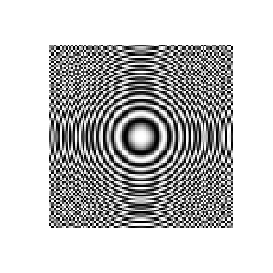
\includegraphics[scale=1]{../imgs/fig2.eps}
	\caption{\textit{zoneplate} subamostrado.}
\end{figure}

\begin{figure}[hbt!]
	\centering
	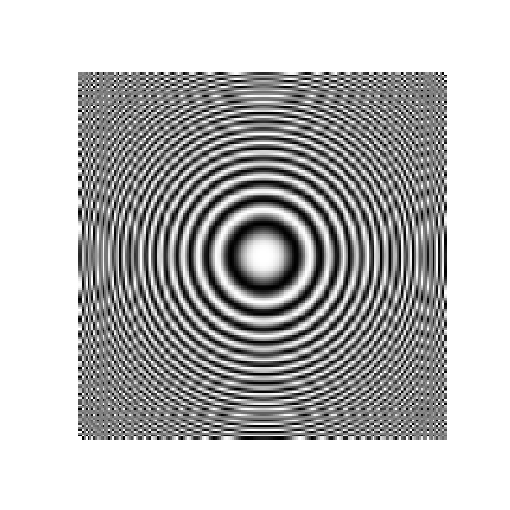
\includegraphics[scale=1]{../imgs/interpol.eps}
	\caption{\textit{zoneplate} interpolado.}
\end{figure}
\item \textbf{Pergunta:} O que você observa no experimento acima?

Podemos observar que a imagem subamostrada possui bordas mais retas, enquanto que a imagem interpolada possui as mesma em degradê. Com as bordas suavizadas, as ilusões causadas pela alta frequência são atenuadas.

\item \textbf{Pergunta:} Por que usar o \textsf{truesize}? Como pode ser explicado o observado nas tarefas acima? 

O \textsf{truesize} mantém as dimensões da imagem. Se a imagem for distorcida os efeitos desejados podem não ser percebidos. Além disso, sem o \textsf{truesize}, a imagem é ampliada, fazendo com que possamos ver as distorções dos pixels.
\end{enumerate}

\end{document}